\section{Introduction}
\label{sect:introduction}

Supersymmetry  (SUSY) \cite{Golfand:1971iw,Wess:1973kz,Wess:1974tw,Fayet1,Fayet2} is one of the most promising extensions of the 
standard model (SM) of elementary particles.  It leads to the unification of gauge couplings at
high energy, it mitigates the problem of quadratic divergences in quantum corrections to the
mass of the Higgs boson, and, in its R-parity-conserving realization, provides a dark matter candidate.
A key prediction of SUSY is the existence of new particles with the same properties as SM particles but
differing in spin by half a unit (``sparticles'').

Extensive searches at the CERN LHC have excluded the existence of colored sparticles with masses below a few hundred \GeV to about 1\TeV,
depending on the details of the assumed models~\cite{%Chatrchyan:2012paa,Chatrchyan:2013xna,Chatrchyan:2013wxa,
Chatrchyan:2013fea,Chatrchyan:2013mys,Chatrchyan:2014aea,Chatrchyan:2014lfa,%Khachatryan:2015exa,
Khachatryan:2015vra,Khachatryan:2015lwa,Aad:2015pfx,Aad:2015iea}. %\cite{susyPhyRes}.
On the other hand, the constraints on sparticles with only electroweak quantum numbers are much less stringent.  This motivates the
work described in this paper.


Searches for charginos, neutralinos, and sleptons by the CMS and ATLAS collaborations are described in Refs.~\cite{Khachatryan:2014qwa,Khachatryan:2014mma,Khachatryan:2015kxa,Aad:2014nua,Aad:2014vma}.
In various SUSY models, the lightest SUSY partners of SM fermions are those from the third generation, 
resulting in enhanced branching fractions for final states with taus~\cite{Martin:1997ns}.  
%Here we report on a search for new physics in events with two $\tau$ leptons and missing transverse momentum (\MPT), i.e., final states that were not explicitly targeted in the previous publications.
The previous searches for charginos, neutralinos,
and sleptons by the CMS collaboration \cite{Khachatryan:2014qwa} are not performed for the case of 
the scalar $\tau$ lepton and its neutrino (\stau and $\sNu_\tau$) 
to be the lightest sleptons. In this paper, a search for charginos is reported using events 
with two opposite-sign $\tau$ leptons and 
missing transverse momentum (\MPT), assuming the masses of the third-generation sleptons are between those of the 
chargino and the lightest neutralino. 
Two $\tau$ leptons can be generated in the decay chain of \sTau 
or charginos (\PSGcpDo) as shown in Fig.~\ref{fig:Productions}. 
\begin{figure}[!htb]
\centering
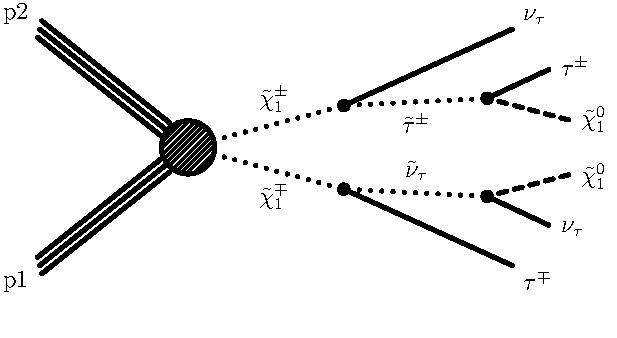
\includegraphics[width=0.49\textwidth]{Introductionfigs/TChipmSlepSnu.pdf}
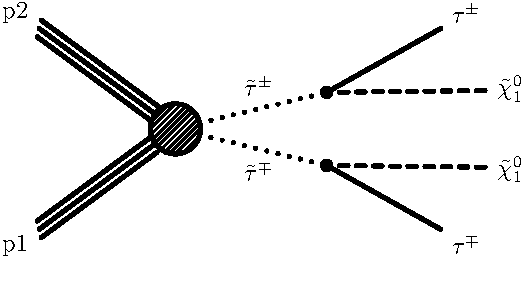
\includegraphics[width=0.49\textwidth]{Introductionfigs/TSlepSlep.pdf}
\caption{Schematic production of double $\tau$ from chargino pair and stau pair.}
\label{fig:Productions}
\end{figure}
%Figure \ref{fig:Productions} shows a representative diagram of pair production of charginos in such a final state. 
The physics interpretation is provided in the context of Simplified Model Spectra (SMS) for SUSY \cite{Alwall:2008ag,alves:sms}.
An ATLAS search for SUSY in di-tau final state is reported in Ref. \cite{Aad:2014yka}, excluding chargino masses up to 345 \GeV 
for a massless neutralino (\PSGczDo).

The results discussed here are based on a dataset of proton-proton 
collisions at $\sqrt{s}$ = 8\TeV
collected with the CMS detector at the CERN LHC during 2012, corresponding to integrated
luminosities of 18.1 and 19.6 \invfb in different channels. 
Our search makes use of the stransverse mass variable (\mttwo)~\cite{Lester:1999tx,Barr:2003rg}
which is the natural extension of transverse mass (\mt) to the case 
where two massive particles with equal mass are created in pairs and decay 
to two invisible particles accompanied by jets and/or leptons.  We consider final states where
two taus are each reconstructed as a hadronic decay of a tau (\tauTau), or where only one tau is reconstructed as the hadronic 
decay of a tau and the other one decays leptonically (\leptonTau;~ $\ell=$ electron or muon).

The paper is organized as follows.  The CMS detector, the event reconstruction, and the data sets are described
in Sections \ref{sect:CMSRec} and \ref{sect:MCSamples}; the \mttwo variable is introduced in Section \ref{sect:mt2def}; 
the event selections for the two channels (\tauTau and \leptonTau)
are described in Sections \ref{sect:tauTauCuts} and \ref{sect:eleTauCuts}, respectively;
a detailed study of the SM backgrounds is presented in Section \ref{sect:bkg}, while Section \ref{sect:sys} 
is devoted to the description of the systematic uncertainties.  The result of the search with its statistical interpretation is presented in 
Section \ref{sect:stat}  
%The main efficiencies of the events selections are summarized in Section \ref{sect:model} 
and the paper is finally summarized in Section \ref{sect:conclusion}.





